\documentclass[tikz]{standalone}
\usetikzlibrary{calc,trees,positioning,arrows,chains,shapes.geometric,%
    decorations.pathreplacing,decorations.pathmorphing,shapes,%
    matrix,shapes.symbols,fit}

\pgfdeclarelayer{back}
\pgfsetlayers{back,main}

\begin{document}
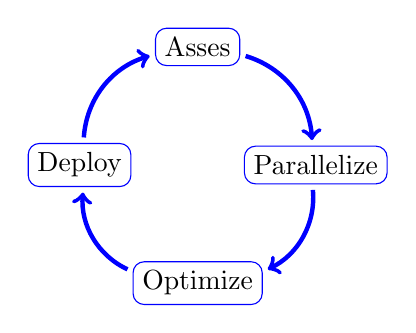
\begin{tikzpicture}[left_arrow/.style={
           ->,
           ultra thick,
           shorten <=2pt,
           shorten >=2pt,
         blue, bend left=35}]

       
  \path (0,3) node(as) [rectangle,rounded corners,draw=blue] {Asses}
  (1.5,1.5) node(par) [rectangle,rounded corners,draw=blue] {Parallelize} 
  (0,0) node(opt) [rectangle,rounded corners,draw=blue] {Optimize} 
  (-1.5,1.5) node(rel) [rectangle,rounded corners,draw=blue] {Deploy} ;
  
  %\draw[thick,red,->] (a) |- +(1,3) -| (c) |- (b);
  \path (as) edge[left_arrow] (par)
  (par) edge[left_arrow] (opt)
  (opt) edge[left_arrow] (rel)
  (rel) edge[left_arrow] (as)
  ;
  
  \end{tikzpicture}
\end{document}
